\documentclass[12pt,a4paper]{article}
\usepackage[utf8]{inputenc}
\usepackage[english]{babel}
\usepackage{enumerate}
\usepackage{amsmath}
\usepackage{amsfonts}
\usepackage{amssymb}
\usepackage{graphicx}
\usepackage{fourier}
\usepackage[left=2cm,right=2cm,top=2cm,bottom=2cm]{geometry}
\usepackage{commath}
\usepackage{cancel}
\usepackage{placeins}
\author{Juan Carlos Apitz, ID 012523821}
\title{STAT572 - Homework Assignment 8}
\begin{document}

\maketitle

\section*{Metropolis-Hastings Sampler for the Beta Distribution}

\textbf{Part a): Random Sample with Beta$\bigr(3,3)$ as target and Unif$\bigr(\theta_1,\theta_2\bigr)$ as proposal.}

\begin{figure}[ht!] 
\begin{center}
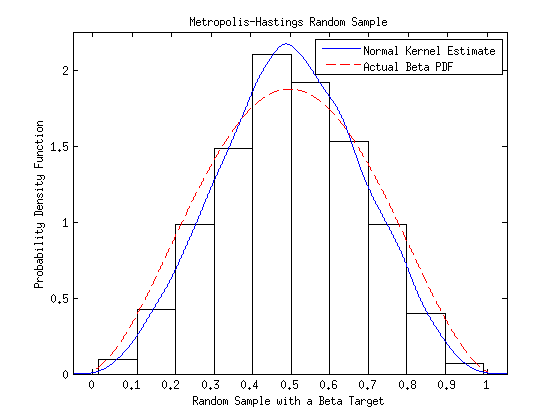
\includegraphics[scale=1]{inclass_graph1.png}
\caption{Histogram of the random sample generated by the Metropolis-Hastings procedure with a target distribution Beta$\bigr(3,3\bigr)$ and a proposal distribution Unif$\bigr(x_{i-1}-0.5, x_{i-1}+0.5\bigr)$. The solid line is the kernel density estimate generated by the normal kernel procedure. The dashed line is the actual graph of the Beta$\bigr(3,3\bigr)$.}
\label{inclass fig1}
\end{center}
\end{figure}
\FloatBarrier
\textbf{Error Measurement:}\\
To get a sense of how well the the sample generated fits the target distribution, we perform a kernel density estimation based on the sample generated and compare this estimate to actual Beta$\bigr(3,3\bigr)$ by calculating: \[\text{ISE}=\int_S\Bigr[\hat{f}(x)-f(x)\Bigr]^2,\]
using the MATLAB numerical integration function trapz() in 100 Monte Carlo trials. Additionally we calculate:
\[\text{MSE}\Bigr[\hat{f}(x_0)\Bigr]=E\Bigr[\hat{f}(x_0)-f(x_0)\Bigr]^2,\]
also in 100 Monte Carlo trials for each value $x_0=0.2,0.5,0.8$. The results are shown below:
\begin{verbatim}
ISE = 0.015723
MSE when xo = 0.2: 0.016787
MSE when xo = 0.5: 0.078622
MSE when xo = 0.8: 0.014729 
\end{verbatim}
It seems the results are reasonable accurate with an approximate level of accuracy $10^{-2}$.\\

\textbf{Part b): Random Sample with Beta$\bigr(3,3)$ as target and Unif$\bigr(\theta_1,\theta_2\bigr)$ as proposal.}
\begin{figure}[ht!] 
\begin{center}
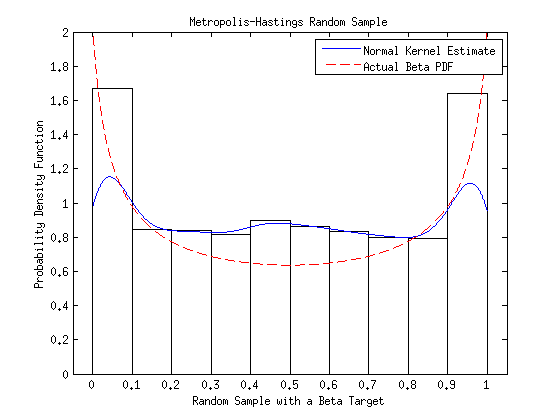
\includegraphics[scale=1]{inclass_graph2.png}
\caption{Histogram of the random sample generated by the Metropolis-Hastings procedure with a target distribution Beta$\bigr(0.5,0.5\bigr)$ and a proposal distribution Unif$\bigr(x_{i-1}-0.5, x_{i-1}+0.5\bigr)$. The solid line is the kernel density estimate generated by the normal kernel procedure. The dashed line is the actual graph of the Beta$\bigr(0.5,0.5\bigr)$.}
\label{inclass fig2}
\end{center}
\end{figure}
\FloatBarrier
\textbf{Error Measurement:}\\
To get a sense of how well the the sample generated fits the target distribution, we perform a kernel density estimation based on the sample generated and compare this estimate to actual Beta$\bigr(0.5,0.5\bigr)$ by estimating the ISE and MSE using the same procedure as in a) above. The results are shown below:
\begin{verbatim}
ISE = 1.903895
MSE when xo = 0.2: 0.002614
MSE when xo = 0.5: 0.068515
MSE when xo = 0.8: 0.002640
\end{verbatim}
The results obtained are not as accurate overall as in part b). The ISE is estimated to 1.9. It is possible this is due to tail behavior of the Beta$\bigr(0.5,0.5\bigr)$. We also observe a consistent deviation from the actual distribution at the mid-point of the distribution. The MSE results at individual point seem more accurate, but still show less accuracy around the middle of the distribution, where $x_0=0.5$.\\

\textbf{Code}
\begin{verbatim}
% METROPOLIS-HASTINGS INCLASS EXERCISE

addpath ~/Documents/Stat572/myfunctions
% Set up function handle to evaluate the Beta.
% Note that in both of the functions, 
% the constants are canceled.
betapdfker = @(x,a,b) (x.^(a-1)).*((1-x).^(b-1));
a = .5; b = .5; % parameters for the beata
% set up function handle to evaluate the proposal distribution
unipdf = @(theta1,theta2) 1./(theta2-theta1);

% 1.GENERATE RANDOM SAMPLE OF SIZE n

% Generate 10000 samples in the chain.
n = 10000; % random sample size
% set up Monte Carlo simulations
M = 100;
ISE = zeros(1,M);
MSE1 = zeros(1,M); MSE2 = zeros(1,M); MSE3 = zeros(1,M);
x0MSE1 = 0.2; x0MSE2 = 0.5; x0MSE3 = 0.8;% to calculate MSE
for j = 1:M
    % initialize the chain
    x = zeros(1,n);
    x(1) = rand(1); % generate the starting point
    for i = 2:n
        % generate a candidate from the proposal distribution. This will be a
        % proposal with parameters given by the previous value in the chain.
        theta1 = max(0,x(i-1)-0.5);
        theta2 = min(x(i-1)+0.5,1);
        y = unifrnd(theta1,theta2,1,1);
        % generate a uniform for comparison
        u = rand(1);
        alphaf = min([1, betapdfker(y,a,b)*unipdf(y-0.5,y+0.5)/...
            (betapdfker(x(i-1),a,b)*unipdf(x(i-1)-0.5,x(i-1)+0.5))]);
        if u <= alphaf
            x(i) = y;
        else
            x(i) = x(i-1);
        end
    end
    % burn-in 5%
    x= x(0.05*n+1:n);
    x0 = min(x)-0.165; xn = max(x)+0.165; % set up domain for kernel estimator
    
    % 2. KERNEL DENSITY ESTIMATION
    
    fhatker = kernelDensEst(x0,xn,x); % my kernel est function
    domain = linspace(x0,xn,5000);
    ISE(j) = trapz(domain,(fhatker-betapdf(domain,a,b)).^2);
    x0ind1 = find(domain>x0MSE1-0.001 & domain<x0MSE1+0.001);
    x0ind2 = find(domain>x0MSE2-0.001 & domain<x0MSE2+0.001);
    x0ind3 = find(domain>x0MSE3-0.001 & domain<x0MSE3+0.001);
    % take mean of MSE because sometimes the x0ind interval may contain 
    % more than one x0
    MSE1(j) = mean((betapdf(x0MSE1,a,b)-fhatker(x0ind1)).^2);
    MSE2(j) = mean((betapdf(x0MSE2,a,b)-fhatker(x0ind2)).^2);
    MSE3(j) = mean((betapdf(x0MSE3,a,b)-fhatker(x0ind3)).^2);
end

% 3. MONTE CARLO SIMULATION OF ISE AND MSE OF RS BASED KERNEL ESTIMATE
ISE = mean(ISE);
MSE1 = mean(MSE1);
MSE2 = mean(MSE2);
MSE3 = mean(MSE3);
fprintf('\nISE = %2.3f',ISE)
fprintf('\nMSE when xo = 0.2: %2.3f',MSE1)
fprintf('\nMSE when xo = 0.5: %2.3f',MSE2)
fprintf('\nMSE when xo = 0.8: %2.3f\n',MSE3)

% 4. PLOT THE RESULTS

[fhath, bc] = hist(x);
fhath = fhath/(0.1*sum(fhath));
bar(bc,fhath,1,'w')
hold on
domain = linspace(min(x)-0.165,max(x)+0.165,5000);
lineker = plot(domain,fhatker);
hold on
linebetapdf = plot(linspace(0,1,5000),betapdf(linspace(0.025,0.975,5000),a,b),'--r');
axis([-0.05 1.05 0 2.2])
xlabel('Random Sample with a Beta Target')
ylabel('Probability Density Function')
title('Metropolis-Hastings Random Sample', 'FontSize',14)
legend([lineker,linebetapdf],'Normal Kernel Estimate','Actual Beta PDF')
hold off
\end{verbatim}
\clearpage

\section*{Metropolis-Hastings Sampler for the Gamma Distribution}
\textbf{Random Sample with Gamma$\bigr(2,3)$ as target and Exponential$\bigr(\beta\bigr)$ as proposal.}

\begin{figure}[ht!] 
\begin{center}
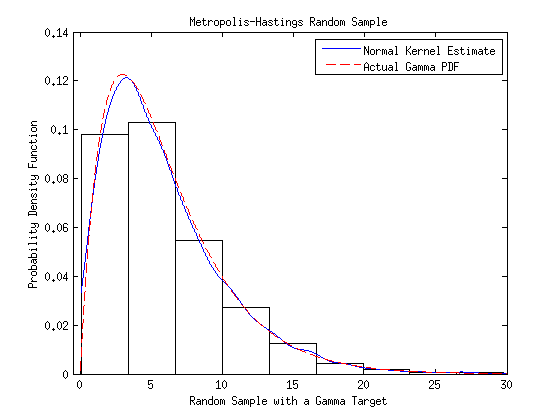
\includegraphics[scale=1]{inclass_graph3.png}
\caption{Histogram of the random sample generated by the Metropolis-Hastings procedure with a target distribution Gamma$\bigr(2,3\bigr)$ and a proposal distribution Exp$\bigr(x_{i-1}\bigr)$. The solid line is the kernel density estimate generated by the normal kernel procedure. The dashed line is the actual graph of the Gamma$\bigr(2,3\bigr)$.}
\label{inclass fig3}
\end{center}
\end{figure}
\FloatBarrier
\textbf{Error Measurement:}\\
To get a sense of how well the the sample generated fits the target distribution, we perform a kernel density estimation based on the sample generated and compare this estimate to actual Gamma$\bigr(2,3\bigr)$ by estimating the ISE and MSE using the same procedure as in the previous exercise above. The results are shown below:
\begin{verbatim}
ISE = 0.000356
MSE when xo = 2: 0.011524
MSE when xo = 5: 0.010846
MSE when xo = 8: 0.003899
\end{verbatim}
It seems the results are reasonable accurate with an approximate level of accuracy $10^{-2}$ for the MSE and $10^{-4}$ for the ISE. This better accuracy is expected as the Gamma and Exponential distributions are closely related as Gamma$\bigr(1,\beta\bigr)\equiv\text{Exponential}\bigr(\beta\bigr)$.

\textbf{Code}
\begin{verbatim}
% METROPOLIS-HASTINGS INCLASS EXERCISE

addpath ~/Documents/Stat572/myfunctions
% Set up function handle to evaluate the Beta.
% Note that in both of the functions, 
% the constants are canceled.
gammapdfker = @(x,a,b) (x.^(a-1)).*exp(-x./b);
a = 2; b = 3; % parameters for the gamma
% set up function handle to evaluate the proposal distribution
exponential = @(x,beta) (exp(-x./beta))./beta;

% 1.GENERATE RANDOM SAMPLE OF SIZE n

% Generate 10000 samples in the chain.
n = 10000; % random sample size
% set up Monte Carlo simulations
M = 100;
ISE = zeros(1,M);
MSE1 = zeros(1,M); MSE2 = zeros(1,M); MSE3 = zeros(1,M);
x0MSE1 = 2; x0MSE2 = 5; x0MSE3 = 8;% to calculate MSE
for j = 1:M
    % initialize the chain
    x = zeros(1,n);
    x(1) = rand(1); % generate the starting point
    for i = 2:n
        % generate a candidate from the proposal distribution. This will be a
        % proposal with parameters given by the previous value in the chain.
        beta = max(0,x(i-1));
        y = exprnd(beta);
        % generate a uniform for comparison
        u = rand(1);
        alphaf = min([1, gammapdfker(y,a,b)*exponential(x(i-1),y)/...
            (gammapdfker(x(i-1),a,b)*exponential(y,x(i-1)))]);
        if u <= alphaf
            x(i) = y;
        else
            x(i) = x(i-1);
        end
    end
    % burn-in 5%
    x= x(0.05*n+1:n);
    x0 = min(x); xn = max(x); % set up domain for kernel estimator
    
    % 2. KERNEL DENSITY ESTIMATION
    
    fhatker = kernelDensEst(x0,xn,x); % my kernel est function
    domain = linspace(x0,xn,5000);
    ISE(j) = trapz(domain,(fhatker-gampdf(domain,a,b)).^2);
    x0ind1 = find(domain>x0MSE1-0.005 & domain<x0MSE1+0.005);
    x0ind2 = find(domain>x0MSE2-0.005 & domain<x0MSE2+0.005);
    x0ind3 = find(domain>x0MSE3-0.005 & domain<x0MSE3+0.005);
    % take mean of MSE because sometimes the x0ind interval may contain 
    % more than one x0
    MSE1(j) = mean((gampdf(x0MSE1,a,b)-fhatker(x0ind1)).^2);
    MSE2(j) = mean((gampdf(x0MSE2,a,b)-fhatker(x0ind2)).^2);
    MSE3(j) = mean((gampdf(x0MSE3,a,b)-fhatker(x0ind3)).^2);
end

% 3. MONTE CARLO SIMULATION OF ISE AND MSE OF RS BASED KERNEL ESTIMATE
ISE = mean(ISE);
MSE1 = mean(MSE1);
MSE2 = mean(MSE2);
MSE3 = mean(MSE3);
fprintf('\nISE = %2.6f',ISE)
fprintf('\nMSE when xo = 2: %2.6f',MSE1)
fprintf('\nMSE when xo = 5: %2.6f',MSE2)
fprintf('\nMSE when xo = 8: %2.6f\n',MSE3)

% 4. PLOT THE RESULTS

[fhath, bc] = hist(x);
fhath = fhath/((bc(2)-bc(1))*sum(fhath));
bar(bc,fhath,1,'w')
hold on
domain = linspace(min(x),max(x),5000);
lineker = plot(domain,fhatker);
hold on
linegammapdf = plot(linspace(0,max(domain),5000),gampdf(linspace(0,max(domain),5000),a,b),'--r');
axis([-0.5 30 0 0.14])
xlabel('Random Sample with a Gamma Target')
ylabel('Probability Density Function')
title('Metropolis-Hastings Random Sample', 'FontSize',14)
legend([lineker,linegammapdf],'Normal Kernel Estimate','Actual Gamma PDF')
hold off
\end{verbatim}
\end{document}